\documentclass[tikz,border=6pt]{standalone}
\usepackage[T1]{fontenc}
\usepackage[utf8]{inputenc}
\usepackage{xcolor}
\usetikzlibrary{arrows.meta,positioning,shapes.geometric}
\definecolor{methodcolor}{HTML}{20913c}
\begin{document}
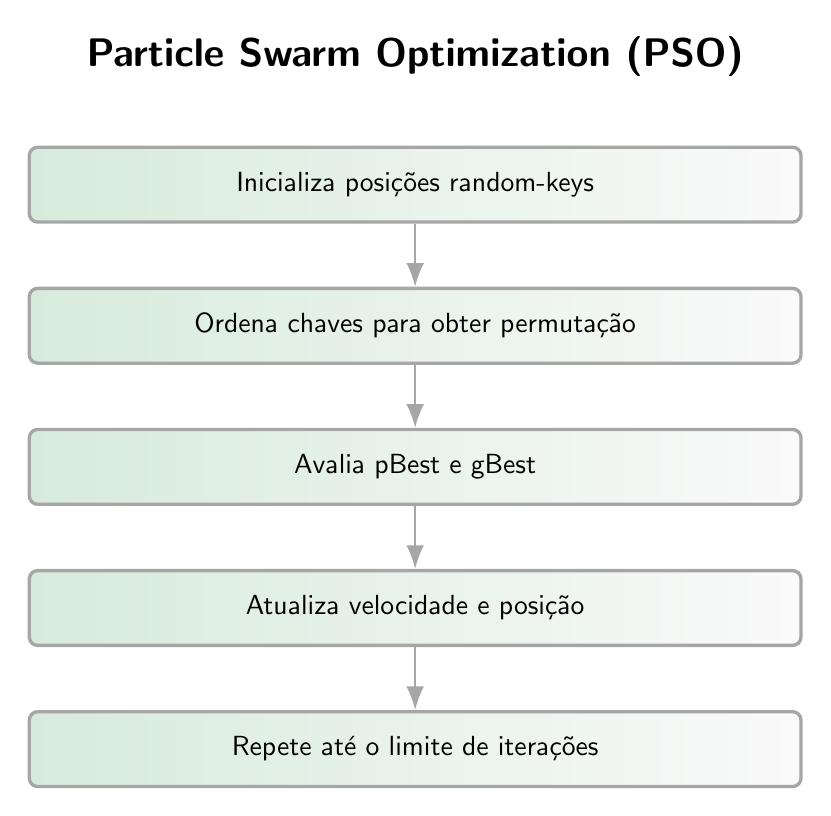
\begin{tikzpicture}[
  font=\sffamily,
  flowbox/.style={rectangle, rounded corners=3pt, draw=gray!70, fill=gray!6, very thick, minimum width=9.8cm, minimum height=0.95cm, align=center, text width=9.2cm, left color=methodcolor!18, right color=gray!4},
  arrow/.style={-{Latex[length=3mm]}, thick, gray!70}
]
\node[font=\sffamily\bfseries\Large] (title) {Particle Swarm Optimization (PSO)};
\node[flowbox, below=0.75cm of title] (step1) {\strut Inicializa posições random-keys};
\node[flowbox, below=0.8cm of step1] (step2) {\strut Ordena chaves para obter permutação};
\node[flowbox, below=0.8cm of step2] (step3) {\strut Avalia pBest e gBest};
\node[flowbox, below=0.8cm of step3] (step4) {\strut Atualiza velocidade e posição};
\node[flowbox, below=0.8cm of step4] (step5) {\strut Repete até o limite de iterações};
\draw[arrow] (step1) -- (step2);
\draw[arrow] (step2) -- (step3);
\draw[arrow] (step3) -- (step4);
\draw[arrow] (step4) -- (step5);
\end{tikzpicture}
\end{document}